\subsection{Database Design}
Databasen bestod i første iteration af individuelle TXT filer som blev brugt som CSV filer. Dette lod os dele dataen op i de forskellige typer af objekter vi gerne ville have opbevaret, f.eks. Episode, Person og Movie, så hver type fik sin egen fil. På den måde undgik vi at indlæse alt vores data når vi skulle have fat i noget specifikt, og dermed spare ressourcer i form af tid og lagring.

\begin{comment}


\begin{figure}[H]
    \centering
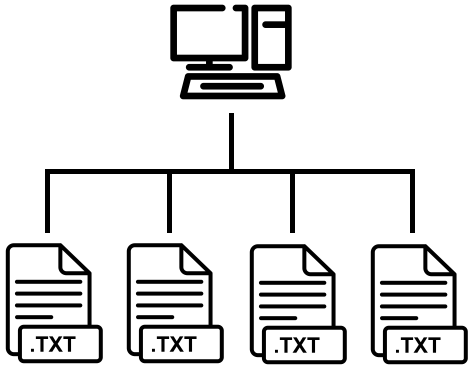
\includegraphics[scale = 0.35]{images/computer_to_txt_file_icon.png}
\caption{Database i form af tekst filer}
\end{figure}

\end{comment}

I anden iteration er der gjort brug af en SQL relationel database, på baggrund af kravene til anden iteration. Ud fra de objekter der findes i systemet har gruppen udarbejdet et UML diagram over databasedesignet, på en sådan måde at det som minimum opfylder 3. normalform. Udarbejdningen af database-strukturen er gjort lettere ved at se på arveheirakiet i programmet, hvor credits er en abstrakt klasse som alle reelle krediterings klasser nedarver fra. På den måde er det lettere at følge arve strukturen og implementere dem til tabeller, hvor der så er gjort brug af foreign keys til at sammensætte de tabeller som i programmet ville extende credits. Andre objekter der ville blive gemt på de forskellige credits, såsom jobs er så også koblet sammen med foreign keys, hvor hvert job er tilknyttet den person som har gjort det, hvilken produktion jobbet er på og hvad jobbet består af. På grund af de tætte tilknytning er der også rig mulighed for at gøre brug af cascade når det er nødvendigt, hvilket gør work-flowet meget mere gennemskueligt når de funktionaliteter implementeres.
UML diagrammet over databasedesignet giver et godt overblik, og viser relationerne mellem de forskellige tabeller, ved crows foot notation. I figur \ref{fig:databaseUML} ses alle tabeller der eksisterer i databasen. Her ses det f.eks. at en "credit" kan have én "person", men at én "person" kan have én eller mange "jobs".
\begin{figure}[H]
    \centering
    \makebox[\textwidth][c]{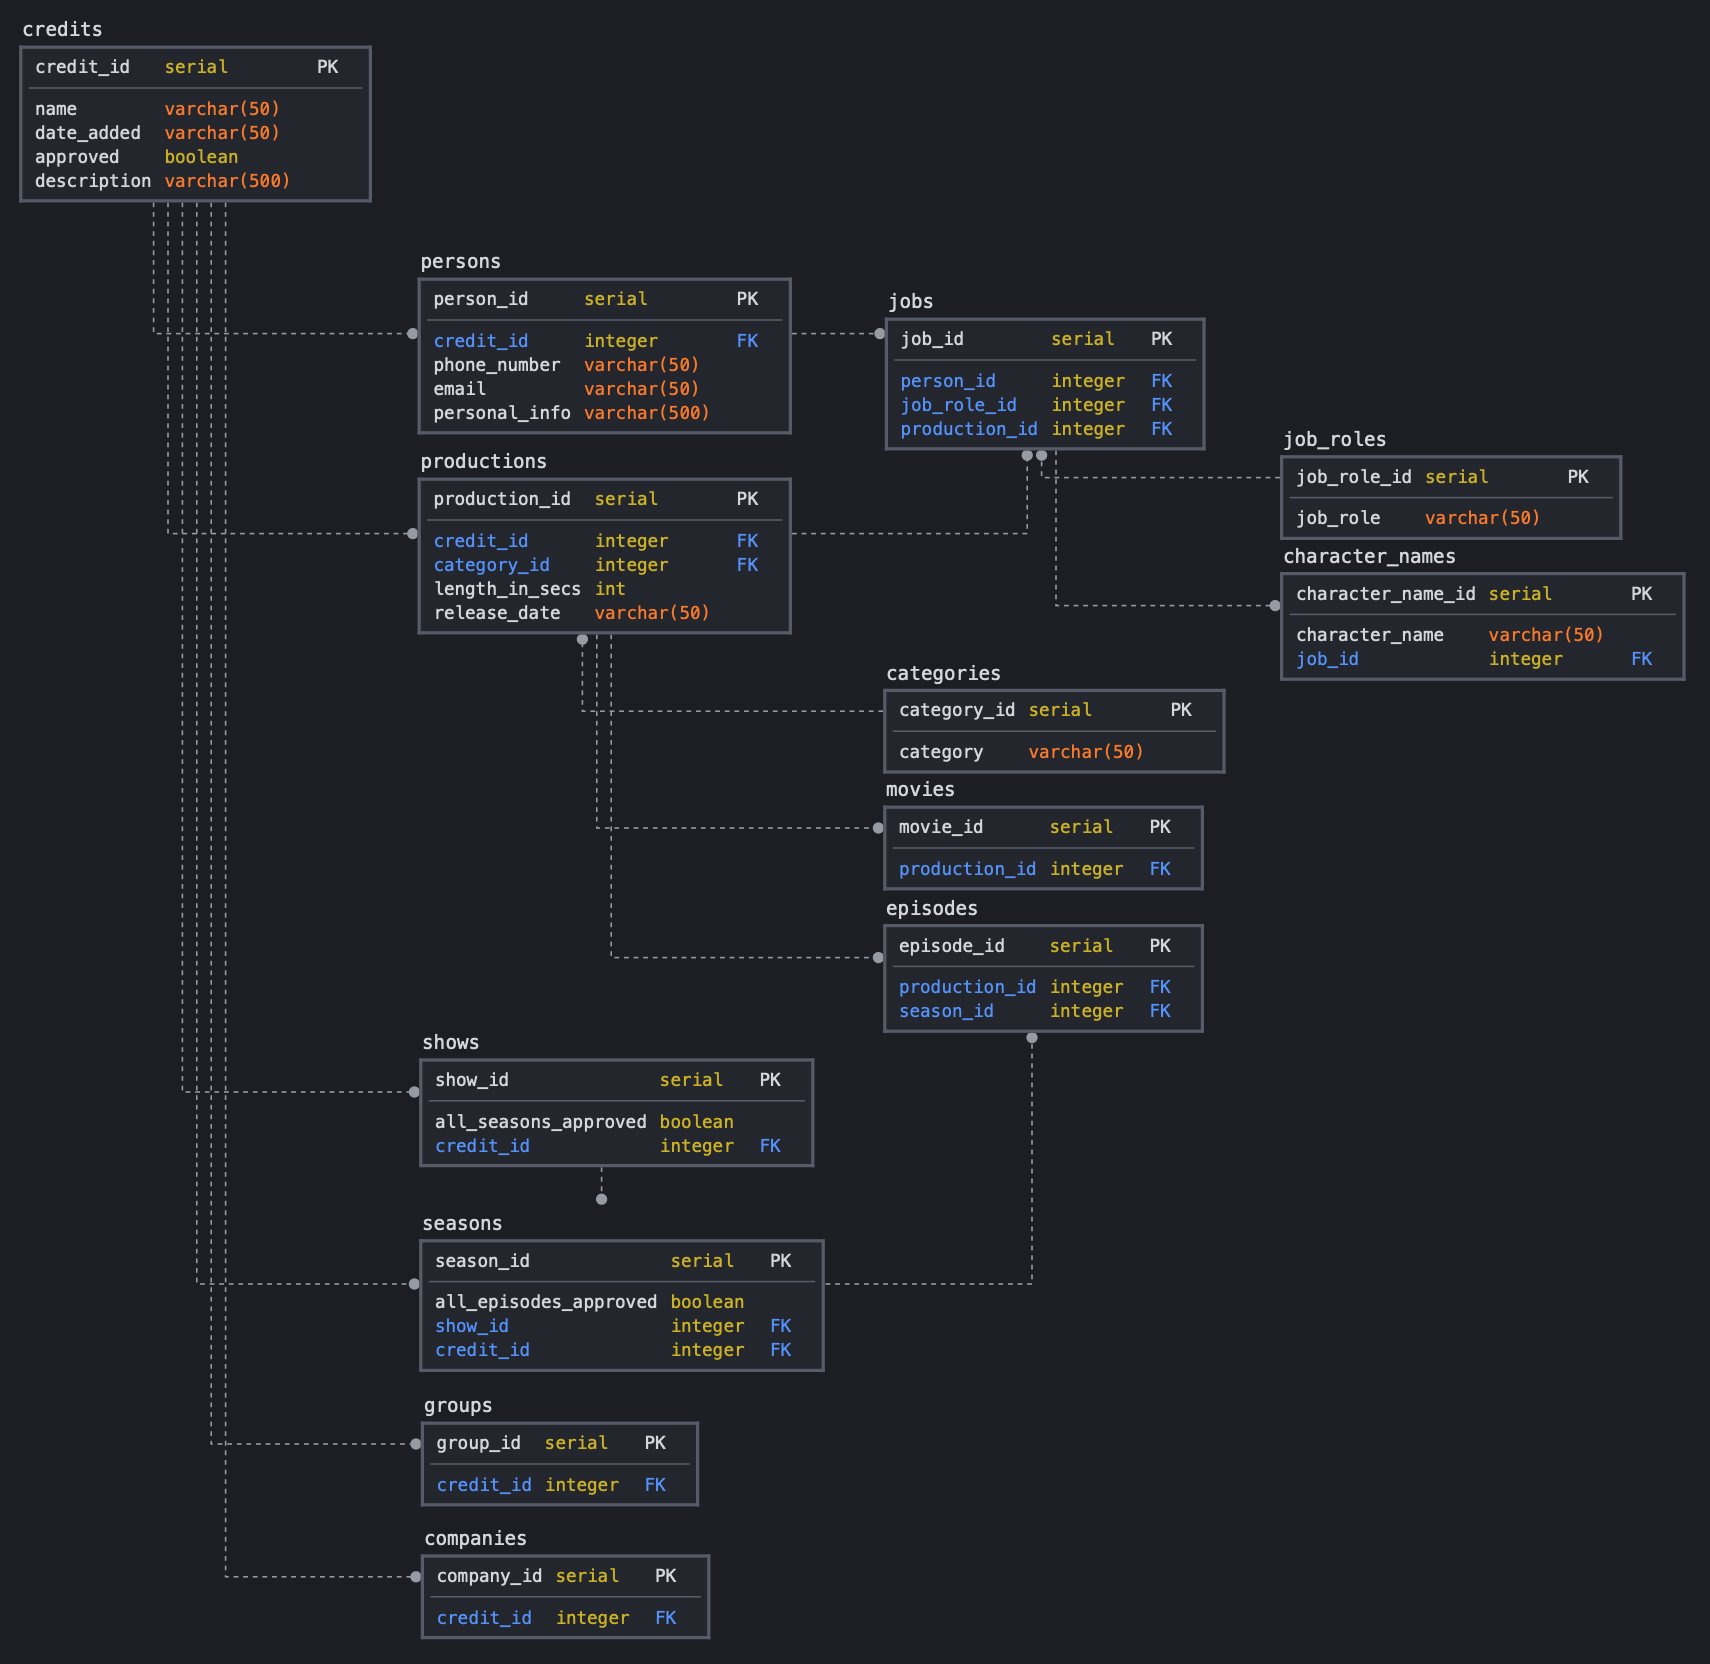
\includegraphics[width=1.25\textwidth]{images/Database design.png}}
    \caption{UML diagram over databasen}
    \label{fig:databaseUML}
\end{figure}